\documentclass[tikz,border=7pt]{standalone}
\usepackage{amsmath}
\usetikzlibrary{arrows.meta}
\begin{document}
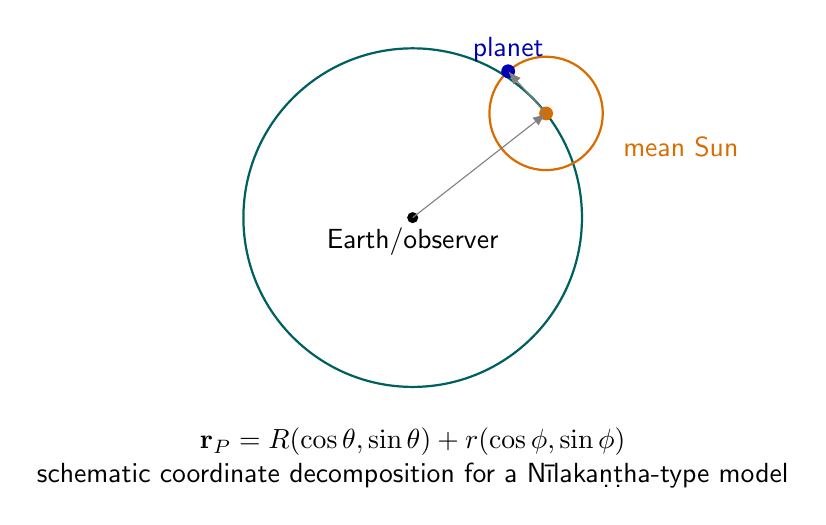
\begin{tikzpicture}[>=Latex,font=\sffamily]
\def\R{2.15}\def\r{0.72}\def\th{38}\def\ph{132}
\coordinate (O) at (0,0);
\coordinate (S) at ({\R*cos(\th)},{\R*sin(\th)});
\coordinate (P) at ({\R*cos(\th)+\r*cos(\ph)},{\R*sin(\th)+\r*sin(\ph)});
\draw[teal!75!black,thick] (O) circle (\R);
\draw[orange!85!black,thick] (S) circle (\r);
\fill (O) circle (2pt) node[below] {Earth/observer};
\fill[orange!85!black] (S) circle (2.5pt);
\node[anchor=west,orange!85!black] at (2.55,.9) {mean Sun};
\fill[blue!70!black] (P) circle (2.5pt) node[above] {planet};
\draw[->,gray] (O)--(S);
\draw[->,gray] (S)--(P);
\node[align=center] at (0,-3.05) {$\mathbf r_P=R(\cos\theta,\sin\theta)+r(\cos\phi,\sin\phi)$\\schematic coordinate decomposition for a N\={\i}laka\d{n}\d{t}ha-type model};
\end{tikzpicture}
\end{document}
